\documentclass[a4paper,12pt]{article}
\usepackage{amsmath, amsthm, amsfonts, amssymb}
\usepackage{mathtools}
\usepackage{microtype}
\usepackage{geometry}
\usepackage{booktabs}
\usepackage{graphicx}
\usepackage{tikz}
\usetikzlibrary{calc}

\newcommand*\diff{\mathop{}\!\mathrm{d}}

\usepackage{caption}
\usepackage{subcaption}
% \geometry{margin=1in}

\usepackage{enumitem}

\usepackage{hyperref}
\usepackage{xcolor}
\hypersetup{ % this is just my personal choice, feel free to change things
    colorlinks,
    linkcolor={red!50!black},
    citecolor={blue!50!black},
    urlcolor={blue!80!black},
}
\usepackage[capitalise]{cleveref}

\usepackage[T1]{fontenc}
\usepackage{sectsty}

\sectionfont{\scshape\mdseries\large}
\subsectionfont{\centering\scshape\bfseries\normalsize}
\subsubsectionfont{\centering\bfseries\small}
\numberwithin{equation}{section}

\colorlet{myred}{red!20}
\colorlet{myblue}{blue!20}
\colorlet{mypurple}{purple!40}
\colorlet{myorange}{orange!20}
\colorlet{myteal}{teal!35}

\DeclarePairedDelimiter\abs{\lvert}{\rvert}%
\DeclarePairedDelimiter\norm{\lVert}{\rVert}%

\newtheorem{theorem}{Theorem}

\title{
    MEK4250\\
    \small{Exam preperation for Finite Elements in Computational Mechanics}
}
\author{August Femtehjell}
\date{Spring 2025}

\begin{document}

\maketitle

\tableofcontents

\begin{abstract}
    This document contains my preperation for the final oral exam for the course MEK4250--Finite Elements in Computational Mechanics, taught at the University of Oslo in the spring of 2025.
    The code for everything, as well as this document, can be found at my GitHub repository: \url{https://github.com/augustfe/MEK4250}.
\end{abstract}

\section*{Exam formalities}
Six problems/topics are given for this exam.
For each problem, the candidate must prepare a 20 minutes oral presentation.
Try to communicate a good overview and understanding of the topic, but compose the talk so that you can demonstrate knowledge about details too.
The student is expected to be able to stick to one subject for the 30 minutes for top grades.
There are no aids besides a whiteboard and this document with the exam problems (experience with this type of exam and various aids tells that learning the content by heart gives by far the best delivery that demonstrates solid understanding).

We will throw a die and the number of eyes determines the topic to be presented.
After your presentation, you will be given some questions, either about parts of your presentation or facts from the other topics.
After each presentation, the next candidate can throw the die and thereby get about 10 minutes to collect the thoughts before presenting the assigned topic.


\section{The finite element method}
Explain Ciarlet's definition of a finite element.
Explain the concept of functionals and function spaces.
How are degrees of freedom used to ensure that the finite element spaces are part of certain function spcaes?
Show that a finite element may conveniently be defined in terms of a reference element.
List common elements in common spaces.

\subsection{Short-form answer}
\subsubsection{Ciarlet's definition}
Ciarlet defined a finite element as a triplet $(T, V, D)$.
Here, $T$ is a bounded domain in $\mathbb{R}^d$, which is typically a polyhedron.
This corresponds to a section of the triangulation of the domain.
Next, $V = \{\psi_i\}_{i = 1}^n$ is a set of linearly independent basis functions defined on $T$.
Finally, $D = \{d_i\}_{i = 1}^n$ is a set of degrees of freedom, which are linear functionals defined on $V$.

We typically want each domain $T$ to be shape regular, i.e.\ such that they are all triangles or all quadrilaterals.
This allows us to perform the computations in a more efficient manner, where we are able to reuse a lot of the computations for each element.
Note that the basis functions $\psi_i$ are only defined locally on the element $T$, and thus they are not defined globally.

The degrees of freedom $d_i$ are what tie the local basis functions together, ensuring properties such as continuity of a certain order across the boundaries of the elements.
With the degrees of freedom, we have the associated \textit{nodal basis} $\{\phi_{i}\}_{i = 1}^n$, which are defined such that
\begin{equation}
    d_j(\phi_i) = \delta_{ij}.
\end{equation}
Finite elements are typically implemented directly through this nodal basis, where the coefficients of the basis functions are defined by the degrees of freedom.

\subsubsection{Functionals and function spaces}
Function spaces are vector spaces, where each element is a function.
Typically, we are looking at function spaces defined through various properties, such as the space of all continuous functions, or the space of all functions with a finite integral.
A functional on a vector space $V$ is then an object $L(\cdot)$, which takes in a vector $v \in V$ and returns a number.
For instance, from a set of coordinates $x_1, x_2, \ldots, x_n$, we can define a functional $L$ on a function space $V = \Span\{\phi_i\}_{i=1}^n$ such that
\begin{equation}
    L(v) = v(x_1) + v(x_2) + \cdots + v(x_n),
    \qquad
    v \in V
\end{equation}
or a set of functionals $L_j$ such that
\begin{equation}
    L_j(\phi_i) = \phi_i(x_j) = \delta_{ij},
    \qquad
    i = 1, 2, \ldots, n.
\end{equation}

Typical function spaces we are interested in the finite element method are Sobolev spaces $W^{k,p}(\Omega)$, which are defined as
\begin{equation}
    W^{k,p}(\Omega) =
    \left\{
        u :
        \left(
            \int_{\Omega}
            \sum_{i \leq k} \abs*{\frac{\partial^i u}{\partial x^i}}^p
            \diff x
        \right)^{1/p} < \infty
    \right\},
\end{equation}
essentially spaces where the function and its derivatives up to order $k$ are in $L^p(\Omega)$.

As far as I'm aware, we are really only interested in the spaces where $p = 2$, which we denote as $H^k(\Omega)$.
The $H$ is chosen after Hilbert, as these are in fact Hilbert spaces.
The inner product for $H^k(\Omega)$ is defined as
\begin{equation}
    (u, v)_{H^k(\Omega)}
    = (u, v)_k
    = \sum_{i \leq k} \int_{\Omega} \frac{\partial^i u}{\partial x^i} \frac{\partial^i v}{\partial x^i} \diff x.
\end{equation}
With the functionals we defined previously, if we choose the points $x_i$ to be along the edges of the elements, we can ensure that they are continuous across elements, which then gives us that the finite element space is a subspace of $H^1(\Omega)$.
Similarly, we can choose a different set of functionals such that we ensure higher order continuity, such as $H^2(\Omega)$.

\subsubsection{Reference element}
In order to illustrate the benefit of a reference element, we consider simply a number of segments of the real number line, with points $x_1 < x_2 < \cdots < x_n$.
Thus, each $T_i$ is simply the segment $[x_i, x_{i+1}]$ for $i = 1, 2, \ldots, n-1$.
On each segment, we have the linear Lagrange basis functions $\phi_i$, which are defined such that $\phi_i(x_j) = \delta_{ij}$.
This is illustrated with $n = 5$ points in \cref{fig:segments}.

\begin{figure}[htbp]
    \centering
    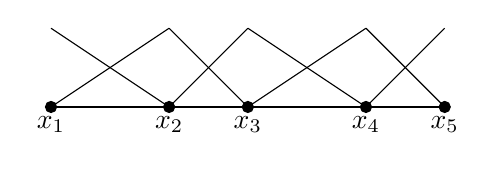
\begin{tikzpicture}
        \def\N{4} % Number of segments
        \foreach \x/\i in {0/1, 1.5/2, 2.5/3, 4/4, 5/5} {
            % Draw a filled circle of radius 2pt at (\x,0) and name that coordinate (x\i)
            \draw[fill=black] (\x,0) circle (2pt) coordinate (x\i);

            % Place the label "x_i" just below the same point (x\i)
            \node[below] at (x\i) {$x_{\i}$};
        }
        \draw[thick] (x1) -- (x\the\numexpr\N + 1\relax);

        \foreach \i in {1,...,\the\numexpr\N\relax} {
            \draw ($(x\i)+(0,1)$) -- (x\the\numexpr\i+1\relax);
            \draw (x\i) -- ($(x\the\numexpr\i+1\relax)+(0,1)$);
        }
    \end{tikzpicture}
    \caption{A number of segments of the real number line, with points $x_1 < x_2 < \cdots < x_n$, defining basis functions $\phi_i$ on each segment.\label{fig:segments}}
\end{figure}

When solving the finite element problem, we typically need to compute matrices $A$ and $M$ defined by
\begin{equation}
    A_{ij} = \int_{\Omega} \nabla \phi_i \cdot \nabla \phi_j \diff x,
    \qquad
    M_{ij} = \int_{\Omega} \phi_i \phi_j \diff x,
\end{equation}
where $A$ is the stiffness matrix and $M$ is the mass matrix.
With the basis functions we have here, these matrices will be incredibly sparse, as for instance $\phi_i$ is only non-zero on the segment $[x_{i-1}, x_{i+1}]$.
As such, we can beforehand say that for instance $A_{1,5}$ will be zero.

We then only need to compute the integrals for the non-zero entries, and we can additionally do this just on each segment, rather than the entire domain.
We are then left with the integrals of the form
\begin{equation}
    A_{ij}
    = \int_\Omega \phi'_i(x) \phi'_j(x) \diff x
    = \int_{x_i}^{x_{i+1}} \phi'_i(x) \phi'_j(x) \diff x
\end{equation}
for $j = i, i+1$.
As of now, we need to compute this for each $i$, however with a change of basis we can instead compute it just once for each segment, getting
\begin{equation}
    A_{j, k}^{(i)} = \int_{0}^{1} \ell'_j(X) \frac{\diff X}{\diff x} \ell'_k(X) \frac{\diff X}{\diff x} \frac{\diff x}{\diff X} \diff X,
\end{equation}
where $X$ is the reference element, and $dX/dx$ is the Jacobian of the transformation from the reference element to the segment.
In the linear case, $\frac{dX}{dx}$ is simply the length of the segment, and we can pull it out of the integral.
Constructing the total stiffness matrix then becomes a matter of computing the integral once for the reference element, and then adding the scaled contributions for each segment.
A similar argument holds for higher order spaces, mapping the physical element to the reference element, however the Jacobian will be more complicated, especially in the case of curved elements.

\subsubsection{Common elements in common spaces}
As mentioned previously, we are mostly interested in the spaces $L^2$, $H^1$ and $H^2$, as well as the spaces $H(\mathrm{div})$ and $H(\mathrm{curl})$.
Let's firstly describe the new spaces $H(\mathrm{div})$ and $H(\mathrm{curl})$.
They are given by
\begin{equation}
    \begin{split}
        H(\mathrm{div}) &= \left\{ u \in L^2(\Omega)^d : \nabla \cdot u \in L^2(\Omega) \right\},\\
        H(\mathrm{curl}) &= \left\{ u \in L^2(\Omega)^d : \nabla \times u \in L^2(\Omega) \right\}.
    \end{split}
\end{equation}

We are typically working with polynomial spaces, which are $C^\infty$ within their domain.
If we allow for discontinuities across the boundaries, we are in $L^2$.
If we enforce continuity across the boundaries, we are in $H^1$, and are typically using Lagrange elements.
If we enforce continuity of the first derivatives as well, we are in $H^2$, and are typically using Hermite elements.
For the spaces $H(\mathrm{div})$ and $H(\mathrm{curl})$, we typically use Raviart-Thomas elements and Nedelec elements respectively.

Raviart-Thomas elements ensure continuity of the normal component across boundaries, while jumps in the tangential component are allowed.
Similarly, as Stokes' Theorem relates curl to the tangential component, Nedelec elements ensure continuity of the tangential component across boundaries, while jumps in the normal component are allowed.

\subsection{Long-form answer}

\subsubsection{Ciarlet's definition of a finite element}
Ciarlet defines a finite element by a triplet $(T, V , D)$, where
\begin{itemize}
    \item
        $T$ is a bounded domain in $R^d$, most typically a polyhedron.

    \item
        $V = \{\psi_i\}_{i = 1}^n$ is a set of linearly independent basis functions on $T$

    \item
        $D = \{d_i\}_{i = 1}^n$ is a set of (linearly independent) degrees of freedom defined in terms of linear functionals on $V$.
        (We remark for $v \in V$ we may evaluate $d_i(v)$ since $d_i$ is a linear functional on $V$.)
\end{itemize}
$T$ defines the triangulation, or cells, in our domain.
The basis functions are then just defined on their cell $T$.
The magic happens when we introduce $D$, dubbed the degrees of freedom, or dofs for short.
They are in a sense how we ``tie'' the function spaces together, as they are originally just defined locally.

Most elements are implemented through a nodal basis, defined by the set of basis functions $\{\phi_i\}_{i = 0}^n$ satsifying $d_j(\phi_i) = \delta_{ij}$.
The simplest example is the Lagrange element, where for a basis function $L_j$, the dofs are defined by
\begin{equation}
    d_i(L_j) = L_j(x_i) = \delta_{ij}.
\end{equation}
Initially, the set $\{x_i\}$ consists of the nodes of each triangle.

Say we have two triangles, each with the vertices $\{x_1, x_2, x_3\}$ and $\{x_4, x_5, x_6\}$ respectively.
If the triangles are next to eachother, we would perhaps then have that $x_2 = x_4$ and $x_3 = x_5$.
However, we still av the set of dofs $\{d_i\}_{i = 1}^{6}$, even though we only have four unique points.
This results in discontinuous Lagrange elements, as they do not directly communicate across the boundaries.
If we however say that $d_2 = d_4$ and $d_3 = d_5$, we would have continuous elements.

\subsubsection{Concept of functionals and function spaces}
A function space is a vector space where each element is a function.
Typically, the function spaces are defined by some properties, for instance the space of all continuous functions, all functions with a finite integral, and especially in our case all functions where the function as well as the derivatives have finite integrals.
This essentially forms our ``main'' space $H^1(\Omega)$, defined by
\begin{equation}
    H^1(\Omega) =
    \left\{
        f
        :
        \int_{\Omega} \abs{f}^2 + \abs{\nabla f}^2 \diff x < \infty
    \right\}.
\end{equation}
A functional is then simply something which takes in a vector, for instance from a function space, and returns a number, either real or complex (although typically real in our case).

\subsubsection{How DOFs define our space}


\section{Weak formulation and finite element error estimation}
\subsection*{Problem description}
Formulate a finite element method for the Poisson problem with a variable coefficient $\kappa : \Omega \to \mathbb{R}^{d \times d}$.
Assume that $\kappa$ is positive and symmetric.
Show that Lax--Milgram's theorem is satisfied. % chktex 8
Consider extensions to e.g.\ convection-diffusion equation and the elasticity equation.
Derive \textit{a priori} error estimates in terms of Cea's lemma for the finite element method in the energy norm.
Describe how to perform an estimation of convergence rates.

\subsection{Short-form answer}
The Poisson problem with a variable coefficient is given by
\begin{equation}
    \begin{split}
        -\nabla \cdot \left( \kappa \nabla u\right) &= f \qquad \text{in } \Omega,\\
        u &= g \qquad \text{on } \partial\Omega_D, \\
        \kappa \frac{\partial u}{\partial n} &= h \qquad \text{on } \partial\Omega_N,
    \end{split}
\end{equation}
where we assume that $\kappa$ is positive, symmetric and bounded.

In order to get the weak form of this problem, we multiply by a test function $v$ and integrate by parts, which yields
\begin{align*}
    \int_\Omega -\nabla \cdot \left( \kappa \nabla u \right) v \diff x
    &= \int_\Omega f \, v \diff x \\
    \int_\Omega \kappa \nabla u \cdot \nabla v \diff x &= \int_{\Omega} f \, v \diff x + \int_{\partial\Omega} \kappa \frac{\partial u}{\partial n} \, v \diff s.
\end{align*}
We can split the boundary integral into two parts, one for the Dirichlet boundary and one for the Neumann boundary:
\begin{align*}
    \int_{\partial\Omega} \kappa \frac{\partial u}{\partial n} \, v \diff s
    &= \int_{\partial\Omega_D}  \kappa \frac{\partial u}{\partial n} \, v \diff s + \int_{\partial\Omega_N} h \, v \diff s \\
    &= \int_{\partial\Omega_D} \kappa \frac{\partial u}{\partial n} \, 0 \diff s + \int_{\partial\Omega_N} h \, v \diff s.
\end{align*}
As the solution is known along the Dirichlet boundary, we can choose $v \in H^1_{0,D}(\Omega)$, which makes the boundary integral there vanish.
This leaves us with the weak form of the Poisson problem, which amounts to finding $u \in H_{g, D}^1(\Omega)$ such that
\begin{equation}
    \int_{\Omega} \kappa \nabla u \cdot \nabla v \diff x = \int_{\Omega} f \, v \diff x + \int_{\partial\Omega_N} h \, v \diff s
    \qquad \forall v \in H^1_{0,D}(\Omega).
\end{equation}
We then get the finite element formulation by discretizing the function space.

For Lax--Milgram to hold, we need to show that: % chktex 8
\begin{align}
    a(u, v) &\leq C_1 \norm{u}_V \norm{v}_V, \qquad \forall u, v \in V, \\
    a(u, u) &\geq C_2 \norm{u}_V^2, \qquad \forall u \in V, \\
    L(v) &\leq C_3 \norm{v}_V, \qquad \forall v \in V,
\end{align}
where $a(u, v)$ is the bilinear form in the weak form, and $L(v)$ is the rhs.

We firstly have
\begin{equation}
    a(u, v) = (\kappa \nabla u, \nabla v)_{L^2} \leq \kappa_{\max} \abs{u}_1 \abs{v}_1 \leq \kappa_{\max} \norm{u}_1 \norm{v}_1,
\end{equation}
where we've used the fact that $\kappa$ is bounded and the Cauchy--Schwarz inequality.

Next, we have
\begin{equation}
    a(u, u) = (\kappa \nabla u, \nabla u)_{L^2} \geq \kappa_{\min} \abs{u}_1^2 \geq C_2 \norm{u}_1^2,
\end{equation}
where we've used the fact that $\kappa$ is bounded below and positive.
We've also used the fact that the $H^1$-norm is equivalent to the $H^1$-semi-norm on $H^1_0$, applying lifting if necessary.

Finally, we have
\begin{align*}
    L(v) &= \int_{\Omega} f \, v \diff x + \int_{\partial\Omega_N} h \, v \diff s \\
    &\leq \norm{f}_{L^2(\Omega)} \norm{v}_{L^2(\Omega)} + \norm{h}_{L^2(\partial\Omega_N)} \norm{v}_{L^2(\partial\Omega_N)} \\
    &\leq C_3 \norm{v}_V,
\end{align*}
assuming we can bound $\norm{v}_{L^2(\partial\Omega_N)}$ by $\norm{v}_1$, and that $f$ and $h$ are bounded.

Extending the equation to the convection-diffusion equation, we simply add the convection term
\begin{equation}
    w \cdot \nabla u = 0
\end{equation}
to the strong form of the equation, which alters the weak form to
\begin{equation}
    a(u, v) = \int_{\Omega} \kappa \nabla u \cdot \nabla v \diff x + \int_{\Omega} w \cdot \nabla u\, v \diff x = \int_{\Omega} f \, v \diff x + \int_{\partial\Omega_N} h \, v \diff s,
\end{equation}
where we've made the assumption that $w$ is bounded.

With the energy norm defined as $\norm{u}_E^2 = a(u, u)$, we have
\begin{align*}
    \norm{u - u_h}_E^2 &= a(u - u_h, u - u_h) \\
    &= a(u - u_h, u - v + v - u_h) \\
    &= a(u - u_h, u - v) + a(u - u_h, v - u_h) \\
    &= a(u - u_h, u - v) + 0 \\
    &\leq \norm{u - u_h}_E \norm{u - v}_E
\end{align*}
which gives us that
\begin{equation}
    \norm{u - u_h}_E \leq \norm{u - v}_E,
\end{equation}
where the choice of $v \in V$ is arbitrary.
Here, we've used Galerkin orthogonality, which states that the error is orthogonal to the finite element space.
Next, choosing $v$ to be the polynomial interpolant of $u$ of degree $t$, we have
\begin{equation}
    \norm{u - I_h u}_E^2 = a(u - I_h u, u - I_h u) \leq \frac{k_1}{1 + C_P} \norm{u - I_h u}_1^2 \leq \frac{k_1}{1 + C_P} (B h^t)^2 \norm{u}_{t+1}^2,
\end{equation}
which yields the error estimate
\begin{equation}
    \norm{u - u_h}_E \leq C h^t \norm{u}_{t+1}.
\end{equation}

With this, we can estimate the convergence rate with elements of a given degree, simply by changing the mesh size $h$, and comparing the error repeatedly.


\subsection{Long-form answer}

\subsubsection{Weak form of the Poisson equation}
The Poisson problem with a variable coefficient $\kappa$ is given by
\begin{equation}
    \begin{split}
        -\nabla \cdot (\kappa \nabla u) &= f \quad \text{in } \Omega, \\
        u &= g \quad \text{on } \partial\Omega_D, \\
        \kappa \frac{\partial u}{\partial n} &= h \quad \text{on } \partial\Omega_N,
    \end{split}
\end{equation}
with $\partial\Omega_D$ and $\partial\Omega_N$ disjoint parts of the boundary $\partial\Omega$.
Here, $\partial\Omega_D$ denotes the Dirichlet boundary, while $\partial\Omega_N$ denotes the Neumann boundary.

Setting up the weak formulation roughly follows the following steps:
\begin{enumerate}
    \item Multiply with a test function $v$ and integrate over the domain $\Omega$

    \item Integrate by parts, and apply Green's lemma.

    \item Apply the boundary conditions.
\end{enumerate}
Multiplying with a test function $v$ and integrating over the domain $\Omega$ gives us
\begin{equation}
    \int_\Omega -\nabla \cdot (\kappa \nabla u) \, v \, \diff x = \int_\Omega f \, v \, \diff x.
\end{equation}
This is however not ideal, as we are now required to have $u \in H^2(\Omega)$, which is not ideal.
We therefore apply Green's lemma to the left-hand side, which gives us
\begin{equation}
    \int_\Omega -\nabla \cdot (\kappa \nabla u) \, v \, \diff x
    = \int_\Omega \kappa \nabla u \cdot \nabla v \, \diff x - \int_{\partial\Omega} \kappa \frac{\partial u}{\partial n} \, v \, \diff s.
\end{equation}
This eases the requirements on $u$, as we now only require $u \in H^1(\Omega)$, while strengthening the requirements on $v$ to $v \in H^1(\Omega)$.

We can now apply the boundary conditions.
Splitting the boundary integral into two parts, we have
\begin{equation}
    \int_{\partial\Omega} \kappa \frac{\partial u}{\partial n} \, v \, \diff s = \int_{\partial\Omega_D} \kappa \frac{\partial u}{\partial n} \, v \, \diff s + \int_{\partial\Omega_N} \kappa \frac{\partial u}{\partial n} \, v \, \diff s.
\end{equation}
As we have a section of Dirichlet boundary, we need not solve for $u$ here, as we know the value of $u$ on this section.
We may therefore set $v = 0$ on $\partial\Omega_D$ by having $v \in H_0^1(\Omega)$, which gives us
\begin{equation}
    \int_{\partial\Omega_D} \kappa \frac{\partial u}{\partial n} \, v \, \diff s + \int_{\partial\Omega_N} \kappa \frac{\partial u}{\partial n} \, v \, \diff s
    = \int_{\partial\Omega_N} h \, v \, \diff s.
\end{equation}

This gives us the weak formulation for the Poisson problem
\begin{equation}
    \int_\Omega \kappa \nabla u \cdot \nabla v \, \diff x = \int_\Omega f \, v \, \diff x + \int_{\partial\Omega_N} h \, v \, \diff s.
\end{equation}

\subsubsection{Lax--Milgram's theorem} % chktex 8
Lax--Milgram's theorem states: % chktex 8
\begin{theorem}
    Let $V$ be a Hilbert space, $a(\cdot, \cdot)$ be a bilinear form, $L(\cdot)$ be a linear form, and let the following three conditions be satisfied:
    \begin{enumerate}
        \item $a(u, u) \geq \alpha \norm{u}_V^2$ for all $u \in V$, where $\alpha > 0$ is a constant.

        \item $a(u, v) \leq C \norm{u}_V \norm{v}_V$ for all $u, v \in V$, where $C > 0$ is a constant.

        \item $L(v) \leq D \norm{v}_V$ for all $v \in V$, where $D > 0$ is a constant.
    \end{enumerate}
    Then, the problem of finding $u \in V$ such that
    \begin{equation}
        a(u, v) = L(v) \quad \forall v \in V
    \end{equation}
    is well-posed in the sense that there exists a unique solution with the stability condition
    \begin{equation}
        \norm{u}_V \leq \frac{C}{\alpha} \norm{L}_{V^*}.
    \end{equation}
\end{theorem}

We can now show that Lax--Milgram's theorem is satisfied for the weak formulation of the Poisson problem. % chktex 8
We have the bilinear form
\begin{equation}
    a(u, v) = \int_\Omega \kappa \nabla u \cdot \nabla v \, \diff x,
\end{equation}
and the linear form
\begin{equation}
    L(v) = \int_\Omega f \, v \, \diff x + \int_{\partial\Omega_N} h \, v \, \diff s.
\end{equation}
We can now show that the three conditions of Lax--Milgram's theorem are satisfied. % chktex 8

Firstly we have that
\begin{align*}
    a(u, u)
    &= \int_\Omega \kappa \nabla u \cdot \nabla u \, \diff x
    = \int_\Omega (\nabla u)^T \kappa^T \nabla u \, \diff x \\
    &= \int_\Omega (\nabla u)^T \kappa \nabla u \, \diff x
    \geq \int_\Omega k_0 \abs{\nabla u}^2 \, \diff x \\
    &= k_0 \abs{u}^2_1
    \geq \alpha \norm{u}_1^2
\end{align*}
where we've first used the fact that $\kappa$ is symmetric, and then that $\kappa$ is positive, and finally that the $H^1_0$ semi-norm is equivalent to the $H^1_0$ norm.

For the second point, we firstly show that $a(\cdot, \cdot)$ defines an inner product, assuming that $\kappa$ is bounded.
The inequality then follows simply from the Cauchy--Schwarz inequality. % chktex 8
In order to show that $a(\cdot, \cdot)$ is symmetric, we simply have
\begin{equation}
    a(u, v) = \int_\Omega \kappa \nabla u \cdot \nabla v \, \diff x
    = \int_\Omega (\nabla v)^T \kappa \nabla u \, \diff x
    = a(v, u).
\end{equation}
We can now show that $a(u, v) \leq C \norm{u}_V \norm{v}_V$.
As $\kappa$ is bounded, we have
\begin{equation}
    \kappa \xi \cdot \xi \leq k_1 \abs{\xi}^2
\end{equation}
for all $\xi \in \mathbb{R}^d$.
This gives us that
\begin{equation}
    a(u, u) = \int_\Omega \kappa \nabla u \cdot \nabla u \, \diff x
    \leq k_1 \int_\Omega \abs{\nabla u}^2 \, \diff x
    \leq k_1 \abs{u}_1^2.
\end{equation}
We then have that
\begin{gather*}
    a(u, v)^2 \leq a(u, u) a(v, v) = k_1^2 \abs{u}_1^2 \abs{v}_1^2 \\
    a(u, v) \leq k_1 \abs{u}_1 \abs{v}_1
\end{gather*}
Additionally, for $H^1_0$ we have
\begin{align*}
    \norm{u}_1^2 = \norm{u}_{L^2}^2 + \abs{u}_1^2
    \leq C \abs{u}_1^2 + \abs{u}_1^2
    = (1 + C) \abs{u}_1^2
\end{align*}
by Poincaré's lemma, which gives us
\begin{equation}
    a(u, v) \leq k_1 \abs{u}_1 \abs{v}_1
    \leq \frac{k_1}{1 + C} \norm{u}_1 \norm{v}_1.
\end{equation}

Lastly, we have
\begin{align*}
    L(v)
    &= \int_\Omega f \, v \, \diff x + \int_{\partial\Omega_N} h \, v \, \diff s
    \leq \norm{f}_{L^2(\Omega)} \norm{v}_{L^2(\Omega)} + \norm{h}_{L^2(\partial\Omega_N)} \norm{v}_{L^2(\partial\Omega_N)} \\
    &\leq (\norm{f}_{L^2}(\Omega) + \norm{h}_{L^2(\partial\Omega_N)}) \norm{v}_{L^2(\Omega)}
    \leq D \norm{v}_{L^2(\Omega)}
    \leq D \norm{v}_1,
\end{align*}
showing that the third condition is satisfied as well.
Here, we assume that $f \in L^2(\Omega)$ and $h \in L^2(\partial\Omega_N)$, which is a reasonable assumption.

\subsubsection{Extension to convection-diffusion equation}
The convection-diffusion equation is given by
\begin{equation}
    \begin{split}
        -\nabla \cdot (\kappa \nabla u) + w \cdot \nabla u &= f \quad \text{in } \Omega, \\
        u &= g \quad \text{on } \partial\Omega_D, \\
        \kappa \frac{\partial u}{\partial n} &= h \quad \text{on } \partial\Omega_N,
    \end{split}
\end{equation}
where $w$ is the convection term.

{\Large To be continued}

\subsubsection{Cea's lemma}
Cea's lemma states that if $u_h$ is the finite element solution, and $u$ is the exact solution, then
\begin{equation}
    \norm{u - u_h}_V \leq \frac{C B}{\alpha} h^t \norm{u}_{t + 1},
\end{equation}
where $B$ is the constant derived from the polynomial approximation, $h$ is a measure of the mesh size, and $C$ and $\alpha$ are constants from Lax--Milgram's theorem. % chktex 8

Here, we assume that the energy norm is given by
\begin{equation}
    \norm{w}_E = a(w, w)^{1/2},
\end{equation}
and that we should find an error estimate in this norm.
We then have
\begin{align*}
    \norm{u - u_h}_E^2 &= a(u - u_h, u - u_h) \\
    &= a(u - u_h, u - v + v - u_h) \qquad v \in V \\
    &= a(u - u_h, u - v) + \underbrace{a(u - u_h, v - u_h)}_{0 \text{ as } v - u_h \in V} \\
    &= a(u - u_h, u - v) \\
    &\leq \norm{u - u_h}_E \norm{u - v}_E.
\end{align*}
Dividing by $\norm{u - u_h}_E$ gives us
\begin{equation}
    \norm{u - u_h}_E \leq \norm{u - v}_E.
\end{equation}
We then further have, choosing $v = I_h u$ as the polynomial approximation of order $t$,
\begin{align*}
    \norm{u - I_h u}_E^2 &= a(u - I_h u, u - I_h u) \\
    &\leq \frac{k_1}{1 + C} \norm{u - I_h u}_1^2 \\
    &\leq \frac{k_1}{1 + C} (B h^t)^2 \norm{u}_{t + 1}^2.
\end{align*}
This finally gives us that
\begin{equation}
    \norm{u - u_h}_E \leq \sqrt{\frac{k_1}{1 + C}} B h^t \norm{u}_{t + 1}.
\end{equation}
I believe this is what the question is asking for, but I am not sure.

\subsubsection{Convergence rates}
We can estimate the convergence rates by looking at the error estimates for varying mesh sizes $h$.
Considering the error estimates for $h = h_1$ and $h = h_2$, we have
\begin{equation*}
    \norm{u - u_{h_1}}_E \leq C h_1^t \norm{u}_{t + 1}
    \quad\text{and}\quad
    \norm{u - u_{h_2}}_E \leq C h_2^t \norm{u}_{t + 1}.
\end{equation*}
This gives
\begin{align*}
    \frac{\norm{u - u_{h_2}}_E}{\norm{u - u_{h_1}}_E}
    &\leq \frac{C h_2^t \norm{u}_{t + 1}}{C h_1^t \norm{u}_{t + 1}} \\
    &= \left(\frac{h_2}{h_1}\right)^t.
\end{align*}
Taking the logarithm of both sides gives us
\begin{align*}
    \log \left(\frac{\norm{u - u_{h_2}}_E}{\norm{u - u_{h_1}}_E}\right)
    &\leq t \log \left(\frac{h_2}{h_1}\right) \\
    \frac{
        \log \left(\frac{\norm{u - u_{h_2}}_E}{\norm{u - u_{h_1}}_E}\right)
    }{
        \log \left(\frac{h_2}{h_1}\right)
    }
    &\leq t.
\end{align*}
If we solve for varying mesh sizes $\{h_i\}_{i=1}^n$, keeping $h_{i+1} / h_i$ constant, we get a series of lower bounds for the convergence rate $t$.

\section{Discretization of Convection-Diffusion}
Derive a proper variational formulation of the convection-diffusion problem.
Derive sufficient conditions that make the problem well-posed.
Discuss why oscillations appear for standard Galerkin methods and show how SUPG methods resolve these problems.
Discuss also approximation properties in light of Cea's lemma.

\subsection{Weak form of the Convection-Diffusion equation}
Here, we consider the convection-diffusion equation given by
\begin{equation}
    \begin{split}
        -\mu \Delta u + w \cdot \nabla u &= f, \quad \text{in } \Omega,\\
        u &= g, \quad \text{on } \partial\Omega,
    \end{split}
\end{equation}
assuming Dirichlet conditions on the whole boundary.

In order to derive the weak form, we follow the steps:
\begin{enumerate}
    \item Multiply the equation with a test function $v$ and integrate.

    \item Integrate by parts, and apply Gauss--Green's lemma. % chktex 8

    \item Apply the boundary conditions.
\end{enumerate}
The first step gives us
\begin{equation}
    \int_\Omega -\mu \Delta u \, v + w \cdot \nabla u \, v \, \diff x = \int_\Omega f \, v \, \diff x.
\end{equation}
Then, we use integration by parts on the first term in order to ease the requirement of $u \in H^2(\Omega)$ to $u \in H^1(\Omega)$, while strengthening the requirement on $v$ from $v \in L_2(\Omega)$ to $v \in H^1(\Omega)$.
This gives us
\begin{equation}
    \int_{\Omega} \mu \nabla u \cdot \nabla v  + w \cdot \nabla u \, v \, \diff x = \int_{\Omega} f \, v \, \diff x + \int_{\partial\Omega} \mu \frac{\partial u}{\partial n} v \, \diff s.
\end{equation}
Next, we consider the boundary term.
As the solution is known on the boundary, we need to solve for $u$ on the boundary, and can therefore choose $v \in H_0^1(\Omega)$, such that
\begin{equation}
    \int_{\partial\Omega} \mu \frac{\partial u}{\partial n} v \, \diff s
    = \int_{\partial\Omega} \mu \frac{\partial u}{\partial n} 0 \, \diff s = 0,
\end{equation}
effectively removing the boundary term from our formulation.

We can now write the weak form of the convection-diffusion equation as
\begin{equation}
    \int_{\Omega} \mu \nabla u \cdot \nabla v + w \cdot \nabla u \, v \, \diff x = \int_{\Omega} f \, v \, \diff x.
\end{equation}
The bilinear form is then given by
\begin{equation}
    a(u,v) = \int_{\Omega} \mu \nabla u \cdot \nabla v + w \cdot \nabla u \, v \, \diff x,
\end{equation}
and the linear form is given by
\begin{equation}
    L(v) = \int_{\Omega} f \, v \, \diff x.
\end{equation}
The weak form of the problem is then, find $u \in V$ such that
\begin{equation}
    a(u,v) = L(v), \quad \forall v \in V.
\end{equation}
% Here, we assume that $\kappa$ is symmetric, positive and bounded, and that $w$ is bounded.

\subsection{Well-posedness}
For well-posedness, we rely on the Lax--Milgram theorem, meaning we have to find sufficient conditions such that: % chktex 8
\begin{enumerate}
    \item $a(u, u) \geq \alpha \norm{u}^2_V$ for some $\alpha > 0$ and all $u \in V$.
    \item $a(u, v) \leq \beta \norm{u}_V \norm{v}_V$ for some $\beta > 0$ and all $u, v \in V$.
    \item $L(v) \leq D \norm{v}_V$ for some $D > 0$ and all $v \in V$.
\end{enumerate}

Here, we'll work through the conditions in reverse order, adding conditions as we go.
For the third condition, we simply have by Cauchy--Schwarz % chktex 8
\begin{equation}
    L(v) = \int_\Omega f \, v \, \diff x \leq \norm{f}_{L^2} \norm{v}_{L^2} \leq \norm{f}_{L^2} \norm{v}_1,
\end{equation}
showing that we require that $f \in L^2(\Omega)$ in order to satisfy the third condition.
For the second condition, we apply lifting to $u$, such that we can use Poincaré's inequality.
We then have
\begin{align*}
    a(u, v)
    &= \int_{\Omega} \mu \nabla u \cdot \nabla v + w \cdot \nabla u \, v \, \diff x \\
    &\leq \mu \abs{u}_1 \abs{v}_1 + \norm{w}_{L^\infty} \abs{u}_1 \norm{v}_{L^2} \\
    &\leq \mu \abs{u}_1 \abs{v}_1 + C \norm{w}_{L^\infty} \abs{u}_1 \abs{v}_1 \\
    &\leq \left( \mu + C \norm{w}_{L^\infty} \right) \abs{u}_1 \abs{v}_1.
\end{align*}
As we've applied lifting to $u$, we can assume that $u \in H^1_0(\Omega)$, such that $\abs{u}_1$ is an equivalent norm to $\norm{u}_1$.

Finally, for the first condition, we write
\begin{equation}
    a(u, v) = b(u, v) + c_w(u, v),
\end{equation}
where $b(u, v) = \int_{\Omega} \mu \nabla u \cdot \nabla v$ and $c_w(u, v) = \int_{\Omega} w \cdot \nabla u \, v$.
For $b$, we already have
\begin{equation}
    b(u, u) = \int_{\Omega} \mu (\nabla u)^2 \, \diff x = \mu \abs{u}_1^2 \geq \frac{\mu}{1 + C} \norm{u}^2_2,
\end{equation}
as
\begin{equation}
    \norm{u}^2_2 = \abs{u}_1^2 + \norm{u}_{L^2}^2 \leq (1 + C) \abs{u}_1^2.
\end{equation}
$c_w$ is a bit more involved, however we start with integration by parts in order to get
\begin{align*}
    c_w(u, v)
    &= \int_{\Omega} w \cdot \nabla u \, v \, \diff x \\
    &= -\int_{\Omega} w \cdot \nabla v \, u \diff x - \int_\Omega \nabla \cdot w \, u \, v \, \diff x + \int_{\partial\Omega} w \cdot n \, u \, v \, \diff s.
\end{align*}
The boundary term vanishes as we've applied lifting, and if we assume that $\nabla \cdot w = 0$ such that we have incompressibility, we are left with
\begin{equation}
    c_w(u, v) = \int_{\Omega} w \cdot \nabla u \, v \, \diff x = -\int_{\Omega} w \cdot \nabla v \, u \diff x = -c_w(v, u).
\end{equation}
$c_w$ is then skew-symmetric, such that we have
\begin{equation}
    c_w(u, u) = -c_w(u, u) = 0.
\end{equation}
The convection-diffusion equation is then well-posed if we assume that $w$ is bounded and incompressible, such that $\nabla \cdot w = 0$.

\subsection{Oscillations in Galerkin methods}
In order to illustrate the oscillations, we consider a simplified scenario in one dimension, where we set $w = -1$.
We then have the equation
\begin{equation}
    \begin{split}
        -\mu u_{xx} - u_x &= 0, \\
        u(0) &= 0, \\
        u(1) &= 1.
    \end{split}
\end{equation}
The variational problem is then, find $u \in H^1_0(0, 1)$ such that
\begin{equation}
    \int_{0}^{1} \mu u_x v_x - u_x v \, \diff x = 0, \quad \forall v \in H^1_0(0, 1).
\end{equation}
Using first order Lagrange elements, we have that the discretization is equivalent to the central finite difference scheme
\begin{equation}
    -\frac{\mu}{h^2} \left[
        u_{i+1} - 2u_i + u_{i-1}
    \right]
    - \frac{w}{2h} \left[
        u_{i+1} - u_{i-1}
    \right] = 0, \quad i = 1, \ldots, N-1,
\end{equation}
which for $\mu = 0$ reduces to $u_{i + 1} = u_{i - 1} = \ldots$ and $u_{i + 2} = u_i = u_{i - 2} = \ldots$.
This is the cause of the oscillations, as if $N$ is odd, then we'll have that all terms of the form $u_{2i} = 0$, while $u_{2i + 1} = 1$, determined by the boundary conditions.

In order to get rid of these oscillations, we can apply upwinding, which amounts to using the approximations
\begin{equation}
    \begin{split}
        \frac{du}{dx}(x_i) &= \frac{1}{h} \left[
            u_{i+1} - u_{i}
        \right] \quad \text{if } w < 0, \\
        \frac{du}{dx}(x_i) &= \frac{1}{h} \left[
            u_{i} - u_{i-1}
        \right] \quad \text{if } w > 0.
    \end{split}
\end{equation}
The oscillations will then dissapear, however we are now using a first order scheme, rather than the second order scheme we had with the central finite difference scheme.
One way to look at this is by noting that
\begin{equation}
    \frac{u_i - u_{i-1}}{h} = \frac{u_{i + 1} - u_{i - 1}}{2h} + \frac{h}{2} \frac{-u_{i + 1} + 2u_i - u_{i - 1}}{h^2},
\end{equation}
as this shows that we are adding a diffusion term with coefficient $\varepsilon = \frac{h}{2}$ to the equation.

This shows that we are then actually solving the problem
\begin{equation}
    -(\mu + \varepsilon) u_{xx} - u_x = f,
\end{equation}
as opposed to the original problem.

\subsection{Streamline diffusion/Petrov--Galerkin} % chktex 8
Streamline diffusion/Petrov--Galerkin (SUPG) methods are a more general and ordered way of dealing with the oscillations we saw in the previous section. % chktex 8
We then add the diffusion in a consistent way, such that we aren't changing the solution as $h \to 0$.

The Petrov--Galerkin method is maybe unsurprisingly very similar to the standard Galerkin method, given by: % chktex 8
Find $u_h \in V_{h,g}$ such that
\begin{equation}
    a(u_h, v_h) = L(v_h), \quad \forall v_h \in W_{h, 0},
\end{equation}
where the difference is that the test space is now different from the trial space.

In matrix form, the Galerkin formulation yields
\begin{equation}
    A_{ij} = a(N_i, N_j) = \int_{\Omega} \mu \nabla N_i \cdot \nabla N_j + w \cdot \nabla N_i \, N_j \, \diff x,
\end{equation}
while the Petrov--Galerkin formulation yields % chktex 8
\begin{equation}
    A_{ij} = a(N_i, L_j) = \int_{\Omega} \mu \nabla N_i \cdot \nabla L_j + w \cdot \nabla N_i \, L_j \, \diff x,
\end{equation}
where $L_j$ is the test function.
Choosing the functions $L_j$ carefully is the key to adding diffusion in a consistent way.

We let $L_j = N_j + \beta h (w \cdot \nabla N_j)$.
This gives us
\begin{align*}
    A_{ij} &= a(N_i, N_j + \beta h (w \cdot \nabla N_j)) \\
    &= \int_{\Omega} \mu \nabla N_i \cdot (N_j + \beta h w \cdot \nabla N_j) \, \diff x + \int_{\Omega} w \cdot \nabla N_i (N_j + \beta h (w \cdot \nabla N_j)) \, \diff x \\
    &= \underbrace{
        \int_{\Omega} \mu \nabla N_i \cdot N_j \, \diff x
        + \int_{\Omega} w \cdot \nabla N_i \, N_j \, \diff x
    }_{\text{Standard Galerkin term}} \\
    &\quad + \underbrace{
        \beta h
        \int_{\Omega} \mu \nabla N_i \cdot \nabla (w \cdot \nabla N_j) \, \diff x
    }_{\text{Vanishes for linear elements}}
    + \underbrace{
        \beta h
        \int_{\Omega} (w \cdot \nabla N_i) (w \cdot \nabla N_j) \, \diff x
    }_{\text{Artificial diffusion in $w$ direction}}.
\end{align*}
The right hand side also changes, denoting the linear form now as $b(L_j)$, such that we have
\begin{equation}
    b(L_j)
    = \int_{\Omega} f L_j \, \diff x
    = \int_{\Omega} f (N_j + \beta h (w \cdot \nabla N_j)) \, \diff x.
\end{equation}
We are in other words changing both sides of the equation, such that the artifical diffusion is consistent.

\subsection{Cea's lemma}
Cea's lemma states that, given the conditions for Lax--Milgram are satisfied, we have % chktex 8
\begin{equation}
    \norm{u - u_h}_{V} \leq \frac{C B}{\alpha} h^t \norm{u}_{t + 1}.
\end{equation}
where $B$ comes the polynomial approximation properties, and $\alpha$ and $C$ are the constants from the Lax--Milgram theorem. % chktex 8
For convection-dominated problems, $\frac{C}{\alpha}$ is large, which causes poor approximation on coarse grids.

In order to get improved error estimates for the SUPG method, we utilize an alternative norm, given by
\begin{equation}
    \norm{u}_{sd} = (h \norm{w \cdot \nabla u}^2 + \mu \abs{\nabla u}^2)^{1/2}.
\end{equation}
Given that the conditions for Lax--Milgram still hold, solving the SUPG problem on a finite element space of order 1 gives us % chktex 8
\begin{equation}
    \norm{u - u_h}_{sd} \leq C h^{3/2} \norm{u}_2.
\end{equation}
The norm $\norm{u}_{sd}$ is called the \textit{streamline diffusion} norm.

The proof for this is very involved, and I'd rather not to too much into detail about it.
One thing to note however is that this error bound is independent of the convection velocity, which is a big improvement over the standard Galerkin method.

\end{document}